\chapter{Theory}
This chapter will develop the relationships between rigid motion, kinematics, velocity and dynamics, \figref{theory_overview}. A strong theoretical foundation of these ideas are elementary for a successful modelling of dynamic behaviour. A successful framework will rely heavily on the theoretical background so the content of the coming chapters will strongly build on the theory presented in this part.

\begin{figure}
 \centering 
 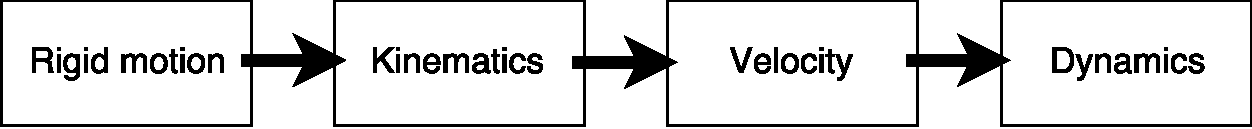
\includegraphics[width=\linewidth]{theory_overview.pdf}
 \caption{Four main parts required to describe the dynamics of a robot}
 \label{theory_overview}
\end{figure}

\section{Rigid motion}
\subsection{Position and rotation}
\subsubsection{Rotations in three dimensions}

If a reference frame $o_0 x_o y_o z_o$ (denoted $O_0$) is rotated in all three dimensions to $O_1$ the \textit{rotation matrix} can be described as the projection of the unit axis in $O_1$ onto $O_0$ as in \eqref{rotmatrix}. This matrix will be used to express point $p^1$ in the reference frame of $O_0$, \eqref{pointrotation}. The same rotation matrix can also be used as an operator to rotate a vector in a fixed reference frame.
\begin{equation}\label{rotmatrix}
R^0_1=\begin{bmatrix}
x_1\cdot x_0 & y_1\cdot x_0 & z_1\cdot x_0\\ 
x_1\cdot y_0 & y_1\cdot y_0 & z_1\cdot y_0\\ 
x_1\cdot z_0 & y_1\cdot z_0 & z_1\cdot z_0
\end{bmatrix}
\end{equation}

\begin{equation}\label{pointrotation}
p^0 = R^0_1p^1
\end{equation}

If $T^0$ is a linear transformation in $O_0$, the same transformation can be expressed in terms if another reference frame $O_1$ as $T^1$ by the help of \eqref{similaritytrans}. This is described as a \textit{similarity transformation} and can be used to express transformation in different reference frames.

\begin{equation}\label{similaritytrans}
T^1 = (R^0_1)^{-1}T^0 R^0_1
\end{equation}

\subsubsection{Composition of rotational transformations}

If $R^0_1$ and $R^1_2$ represents rotational transformations between reference frames \textit{0, 1} and \textit{1, 2}. Then point $p^2$ can be described in terms of $O_0$ as in \eqref{rotationcomposition}. This will be rotation with respect to the \textit{current frame}, which will change as as the transformation happen. If a \textit{fixed axis rotation} is wanted instead, the rotation composition has to be pre multiplied instead of post multiplied, shown in \eqref{rotationcomposition_pre}. As a result it is possible to find a single rotation matrix \textit{$R^i_n$} which describes the combination of an infinite amount of dependent rotations from \textit{i} to \textit{n}, \eqref{Rcompositioninf}.


\begin{equation}\label{rotationcomposition}
p^0 = R^0_1 R^1_2 p^2
\end{equation}

\begin{equation}\label{rotationcomposition_pre}
p^0 = R^1_2 R^0_1 p^2 = R R^0_2 p^2
\end{equation}

\begin{equation}\label{Rcompositioninf}
R^i_n = \prod_{i=0}^{n-1} R^i_{i+1}
\end{equation}


\subsubsection{Parametrisation of rotations}

In equation \eqref{rotmatrix} the transformation were described in terms of nine independent variables. A rotation in 3D can at most have three independent variables and it is therefore convenient to perform a parametrization to get three independent variables. This can be done by using \textit{euler angles}, \textit{roll pitch yaw} or \textit{axis/angle} representation. The euler angle rotation is rotation about ZYZ axis by an amount $\phi, \theta, \psi$ respectively, see \eqref{eulertrans}. \textit{C} and \textit{s} represents the cosine and sine functions respectively. Yaw, Pitch and Roll rotations are rotations around XYZ relative to a fixed frame an described in \eqref{ywapitchroll}.
\begin{align}\label{eulertrans}
\begin{split}
R_{ZYZ} &= R_{z,\phi}R_{y,\theta}R_{z,\psi} \\
&= \begin{bmatrix}
c_\phi c_\theta c_\psi - s_\phi s_\psi & -c_\phi c_\theta s_\psi - s_\phi c_\psi & c_\phi s_\theta\\ 
s_\phi c_\theta c_\psi + c_\phi s_\psi & -s_\phi c_\theta s_\psi + c_\phi c_\psi  & s_\phi s_\theta \\ 
-s_\theta c_\psi & s_\theta s_\psi & c_\theta
\end{bmatrix}
\end{split}
\end{align}


\begin{align}\label{ywapitchroll}
\begin{split}
R_{XYZ} &= R_{z,\phi}R_{y,\theta}R_{x,\psi} \\
&= \begin{bmatrix}
c_\phi c_\theta & - s_\phi c_\psi + c_\phi s_\theta s_\psi & s_\phi s_\psi + c_\phi s_\theta c_\psi \\ 
s_\phi c_\theta & c_\phi c_\psi + s_\phi s_\theta s_\psi  & - c_\phi s_\psi + s_\phi s_\theta c_\psi \\ 
-s_\theta & c_\theta s_\psi & c_\theta c_\psi
\end{bmatrix}
\end{split}
\end{align}

If $R_{k,\theta}$ describes the rotation about a unit vector $k$ with an angle $\theta$ we get what is called an \textit{axis/angle} rotation. If $R$ is the rotation transformation that aligns the z-axis with $k$, \eqref{similaritytrans} can bu used to derive $R_{k,\theta}$ as in \eqref{axisanglerot}.

\begin{equation}\label{axisanglerot}
R_{k,\theta} = R^{-1} R_{z,\theta} R
\end{equation}

\subsection{Rigid motion}

Rigid motion is a combination of rotation and translation. The matrix form is described as a \textit{homogeneous transformation} and is defined as a set of matrices as in \eqref{homeqn}. \textit{R} is the rotation matrix as described before and \textit{d} is the translation vector with respect to a chosen base frame. The same features of composition as described in \eqref{Rcompositioninf} also applies to homogeneous transformation.

\begin{equation}\label{homeqn}
H = \begin{bmatrix}
R_{3x3} & d_{3x1}\\ 
0_{1x3} & 1_{1x1}
\end{bmatrix}
\end{equation}


\section{Kinematics}

To describe the dynamics in a serial manipulator or robots in general it's kinematic relationships has to be used. In this section the forward and inverse kinematics will be described shortly and will form the basis for velocity kinematics and dynamics.

\subsection{Denavit-Hartenberg convention}

The homogeneous transformation as described in \eqref{homeqn} is a matrix of six independent variables. But introducing two constraints on how the reference frames are defined with respect to each other the total number of independent variables can be reduced to four. This is the motivation behind the \textit{\gls{DH}} (DH). This convention also provides a common, well known framework for defining robotic systems among engineers.

A DH transformation is defined as a product of four basic transformations, \eqref{DH}. Where $a_i, \alpha_i, d_i $ and $\theta_i$ represents the link length, link twist, link offset and joint angle respectively, for link number \textit{i}. The transformation from the rigid base frame $0$ to the end effector $n$ will then be the product sum of the transformations for each link, \eqref{DHsum}.

\begin{align}\label{DH}
\begin{split}
A_i &= Rot_{z,\theta_i}Trans_{z,d_i}Trans_{x,a_i}Rot_{x,\alpha_i} \\
&= \begin{bmatrix}
c_{\theta_i} & -s_{\theta_i}c_{\alpha_i} & s_{\theta_i}s_{\alpha_i} & a_{i}c_{\theta_i} \\ 
s_{\theta_i} & c_{\theta_i}c_{\alpha_i} & -c_{\theta_i}s_{\alpha_i} & a_{i}s_{\theta_i} \\ 
0 & s_{\alpha_i} & c_{\alpha_i} & d_i \\ 
0 & 0 & 0 & 1 
\end{bmatrix}
\end{split}
\end{align}

\begin{equation}\label{DHsum}
T^0_n=\prod_{i=1}^{n}A_i
\end{equation}

In essence, this establishes the forward kinematic relationship. Each link in the robot can be defined as in \eqref{DH} where either $\theta_i$ or $d_i$ is the varying variable depending on the joint is revolute or prismatic. Lastly, \eqref{DHsum} will give the position and rotation of the end effector with respect to the base frame.

\subsection{Inverse kinematics}

\section{Velocity kinematics}
\lipsum[1]
\subsection{Jacobian}
\subsection{Force and torque relationships}
\subsection{Inverse velocity and acceleration}

\section{Dynamics}
\lipsum[1]
\subsection{Euler-Lagrange equations}
\subsection{Kinetic and potential energy}
\subsection{Newton euler formulation}